% =============================================================================
%  Structured Memory and Selective Agreement in Populations of LLM Agents
%  Single-file manuscript for Overleaf / Prism. Upload this file together with
%  references.bib and the four figure PNGs (keep them in the same folder).
%
%  How to read this file
%  - Lines starting with "% GUIDE" are writing guidance for the section below
%    them. Delete each GUIDE block once the section is written.
%  - Tables and figures are already typeset with verified numbers. Keep, move,
%    edit, or delete them as your text requires.
%  - Every number you write must come from reports/full_ablation_summary.md
%    (in the project repository), and every citation from references.bib.
%  - \pending{...} prints in red: use it for anything unresolved.
%  - Full background: paper/context/README.md in the repository.
% =============================================================================

\documentclass[11pt,a4paper]{article}
% Venue (EPJ Data Science, class sn-jnl) is not confirmed yet. Keep `article`
% until it is; switching later only touches this preamble.

\usepackage[utf8]{inputenc}
\usepackage[T1]{fontenc}
\usepackage{lmodern}
\usepackage[margin=2.5cm]{geometry}
\usepackage{amsmath,amssymb}
\usepackage{graphicx}
\usepackage{booktabs}
\usepackage{array}
\usepackage{tabularx}
\usepackage[hyphens]{url}
\usepackage[font=small,labelfont=bf]{caption}
\usepackage[round,authoryear]{natbib}
\usepackage{xcolor}
\usepackage{microtype}
\usepackage[hidelinks]{hyperref}

\newcommand{\pending}[1]{\textcolor{red}{\textbf{[#1]}}}   % unresolved item
\newcommand{\cond}[1]{\textsf{#1}}                         % condition name, e.g. \cond{no\_kg}

\title{Structured Memory and Selective Agreement\\in Populations of LLM Agents}
\author{Pranav Deepak \and Giulio Rossetti\\[0.5em]
  \small\pending{author order, affiliations, corresponding author}}
\date{Draft of \today}

\begin{document}
\maketitle

% =============================================================================
\begin{abstract}
% GUIDE  Write this LAST, after the Discussion and Conclusion.
% GUIDE  150-250 words, one paragraph: (1) the LODAS finding you extend,
% GUIDE  (2) the gap (no memory), (3) what you did (GhostKG + FSRS, four
% GUIDE  conditions, 140 agents, 30 days, shared pairing schedule), (4) the
% GUIDE  three findings with one or two numbers, (5) the reversed prediction,
% GUIDE  (6) the single-run caveat.
% GUIDE  Headline numbers: directional bias +0.176 (general_only) vs +0.042
% GUIDE  (no_kg); churn 47.9% (full_kg) vs 26.7-33.6%. Summary file, Sections 2.2, 3.4.
\pending{abstract}
\end{abstract}

% =============================================================================
\section{Introduction}\label{sec:intro}
% GUIDE  Purpose: from single-model sycophancy, to population-level selective
% GUIDE  agreement, to the open question about memory.
% GUIDE  Suggested paragraphs:
% GUIDE   1. Single-agent sycophancy: perez2023discovering, sharma2023sycophancy,
% GUIDE      wei2023synthetic.
% GUIDE   2. LODAS and selective agreement (cau2025selective). Selective agreement is
% GUIDE      DIRECTIONAL: acceptance rises with signed distance toward the framing
% GUIDE      statement. It is not "agents accept nearby partners".
% GUIDE   3. LODAS agents have no memory; memory is central to LLM agents
% GUIDE      (zhang2025memorysurvey, park2023generative).
% GUIDE   4. What you do: GhostKG (ghostkg) with FSRS decay (fsrs_algorithm,
% GUIDE      ye2022ssp, su2023dynamics); four conditions.
% GUIDE   5. Prediction vs finding, in two sentences.
% GUIDE   6. A contributions list (itemize), then a one-line roadmap.
% GUIDE  Avoid: "larger scale than LODAS" (LODAS also used 140 agents) and
% GUIDE  "the +/-1 rule is novel" (LODAS already updates by +/-1).
% GUIDE  Length: about 700 words. Revise after the Discussion is written.
\pending{introduction}

% =============================================================================
\section{Related Work}\label{sec:related}
% GUIDE  Cite ONLY keys in references.bib; each key's allowed claims are listed in
% GUIDE  paper/context/related_work_sources.md ("Supports:" lines).
% GUIDE  Need a paper that isn't there? Ask the lit-scout / citation-verifier
% GUIDE  agents (see the README) instead of citing from memory.
% GUIDE  Length: 900-1300 words.

\subsection{Opinion dynamics models and their metrics}\label{sec:related-od}
% GUIDE  degroot1974consensus, hegselmann2002opinion, deffuant2000mixing,
% GUIDE  holley1975ergodic, castellano2009statistical, sirbu2017opinion.
% GUIDE  End with: our entropy, cluster, and acceptance metrics follow cau2025selective.
\pending{write}

\subsection{Sycophancy in single-agent settings}\label{sec:related-syco}
% GUIDE  perez2023discovering, sharma2023sycophancy, wei2023synthetic; then how
% GUIDE  cau2025selective separates selective agreement from sycophancy (their
% GUIDE  Llama agents show "a form of bounded confidence").
\pending{write}

\subsection{LLM agent populations as opinion-dynamics simulators}\label{sec:related-pop}
% GUIDE  chuang2024simulating; LODAS facts (verified from the full text): 7-point
% GUIDE  scale, the Discussant updates ITSELF (no annotator), Ship of Theseus with a
% GUIDE  framing statement, Mistral-7B and Llama-3-8B, 140 agents, 30 iterations,
% GUIDE  10 runs, about 20% of statements fallacious.
\pending{write}

\subsection{Memory for LLM agents}\label{sec:related-mem}
% GUIDE  lewis2020rag, park2023generative, packer2023memgpt, zhong2024memorybank
% GUIDE  (Ebbinghaus-inspired forgetting: your closest contrast),
% GUIDE  zhang2025memorysurvey, edge2024graphrag (cite only for existence).
% GUIDE  Close with the gap: nobody varies the KIND of memory while holding the
% GUIDE  population, pairing schedule, and topic fixed.
\pending{write}

% =============================================================================
\section{Method}\label{sec:method}
% GUIDE  Source for every sentence: paper/context/methodology_facts.md. If a
% GUIDE  mechanism is not in that file, check the code and add it there first.
% GUIDE  Length: 1400-1900 words.

\subsection{Simulation framework}\label{sec:method-sim}
% GUIDE  Cadence: do NOT write "once per day". Approved wording (methodology_facts.md):
% GUIDE  "In the delivered runs, each agent initiated one exchange per simulated hour
% GUIDE  with a uniformly random partner, for 24 rounds per simulated day over 30
% GUIDE  days. This cadence is recovered from the logged data; the exact loop
% GUIDE  implementation used on the collaborator's infrastructure is pending
% GUIDE  confirmation."
% GUIDE  Also: 2-5 turns per exchange; a separate annotator reads only the scored
% GUIDE  agent's utterances; both participants are scored; identical pairing
% GUIDE  schedule and turn counts across conditions (common random numbers).
% GUIDE  State the three differences from LODAS (annotator, 5 vs 7 points, topic).
\pending{write}

\subsection{Stance scale and the one-step rule}\label{sec:method-clamp}
% GUIDE  Clamp: new = max(prev - 1, min(prev + 1, proposed)). Same +/-1 rule as
% GUIDE  LODAS, but enforced on the annotator output. No delivered update moves
% GUIDE  more than one step.
\pending{write}

\subsection{Memory conditions}\label{sec:method-memory}
% GUIDE  AgentMemory interface; NullMemory (no_kg); GhostMemory with a dimensions
% GUIDE  list (table below). "tom" here means one thing only: an inferred belief
% GUIDE  about what a specific partner believes, stored as a triplet.
\pending{write}

\begin{table}[t]
\centering
\small
\caption{Knowledge-graph dimensions active in each memory condition.}
\label{tab:dims}
\begin{tabular}{lc}
\toprule
Condition & dimensions \\
\midrule
\cond{general\_only} & [``general''] \\
\cond{tom\_only} & [``tom''] \\
\cond{full\_kg} & [``general'', ``tom'', ``beliefs''] \\
\bottomrule
\end{tabular}
\end{table}

\subsection{GhostKG mechanics}\label{sec:method-ghostkg}
% GUIDE  One extraction call per active dimension, 0-5 (s, p, o) triplets; only
% GUIDE  (s, p, o) is stored, the round field is stripped; FSRS-6 decay on the
% GUIDE  simulated clock via set_agent_time(); default parameters, untuned;
% GUIDE  GhostKG 0.2.0. How often the clock was advanced in the DGX runs is
% GUIDE  \pending.
\pending{write}

\subsection{Population, topic, and stance polarity}\label{sec:method-pop}
% GUIDE  140 personas, 14/28/56/28/14, stance tied to the persona.
% GUIDE  Polarity: the persona file intends In Favor = supports RESTRICTIVE
% GUIDE  immigration policy, but the prompts give only the topic string and never
% GUIDE  state a proposition. So report stances by scale label only. Never write
% GUIDE  "pro-immigration" or "anti-immigration".
\pending{write}

\subsection{Metrics}\label{sec:method-metrics}
% GUIDE  Entropy H(t) in bits; effective clusters C = 1/sum p_i^2; acceptance on
% GUIDE  SIGNED distance Delta x = x_partner - x_agent (cau2025selective) and the
% GUIDE  asymmetry P(A|+k) - P(A|-k); unsigned d = |Delta x| and move-away rate;
% GUIDE  per-stance mobility; mean stance score. Analysis script:
% GUIDE  scripts/compute_paper_numbers.py. Agent-clustered bootstrap (1,000
% GUIDE  resamples of 140 agents) = WITHIN-RUN variability only.
\pending{write}

\subsection{Model and infrastructure}\label{sec:method-model}
% GUIDE  vLLM on the collaborator's DGX. Model: \pending until Rossetti confirms.
% GUIDE  Do not name Llama-3.1 or llama3.2.
\pending{write}

% =============================================================================
\section{Experimental Setup}\label{sec:setup}
% GUIDE  Length: 500-800 words.
% GUIDE  1. The ablation: 4 conditions x 1 run, seed 42, 720 rounds, 100,800
% GUIDE     exchanges per condition (403,200 total), 201,600 scored updates per
% GUIDE     condition. Summary file, Section 1.
% GUIDE  2. Research question and hypothesis exactly as in
% GUIDE     paper/context/hypothesis_and_scope.md, with its support/against
% GUIDE     criteria, described as "stated in advance in an internal document"
% GUIDE     (it was NOT a formal pre-registration). No outcomes here.
% GUIDE  3. LODAS vs this study: the table below.
% GUIDE  4. The 10-day llama3.2/Ollama pilot: mention it; never pool its numbers.
% GUIDE  5. Not run: second topic, neutral control, cross-model, annotator context.
\pending{write}

\begin{table}[t]
\centering
\small
\caption{Design of LODAS \citep{cau2025selective} compared with this study.}
\label{tab:lodas}
\begin{tabularx}{\linewidth}{>{\raggedright\arraybackslash}p{0.28\linewidth}>{\raggedright\arraybackslash}X>{\raggedright\arraybackslash}X}
\toprule
Property & LODAS (Cau et al. 2025) & This study \\
\midrule
Scale points & 7 & 5 \\ \addlinespace
Who updates & Discussant updates itself, no separate annotator & A separate annotator scores both participants \\ \addlinespace
Topic & Ship of Theseus, with an explicit framing statement & Immigration policy, no stated proposition \\ \addlinespace
Models & Mistral-7B-Instruct and Llama-3-8B & Pending confirmation \\ \addlinespace
Runs & 10, averaged & 1 per condition \\ \addlinespace
Agents & 140 & 140 \\ \addlinespace
Horizon & 30 iterations of N pairwise interactions & 30 simulated days of 24 rounds of N exchanges \\ \addlinespace
Memory & None & Four conditions: none, general facts, theory-of-mind, combined \\
\bottomrule
\end{tabularx}
\end{table}

% =============================================================================
\section{Results}\label{sec:results}
% GUIDE  The ONLY source of numbers: reports/full_ablation_summary.md. Copy values
% GUIDE  exactly; do not round or derive new ones. Say once that the intervals are
% GUIDE  within-run and agent-clustered (one run per condition).
% GUIDE  Report signed acceptance (Cau's definition) BEFORE unsigned.
% GUIDE  Length: 1800-2400 words.

\subsection{Population-level outcomes}\label{sec:res-pop}
% GUIDE  Summary file, Sections 2.1-2.2. Neutral and both extremes collapse within
% GUIDE  day 1, then fluctuate. general_only is the most convergent, full_kg the
% GUIDE  most dispersed and the highest churn (47.9%).
\pending{write}

\begin{table}[t]
\centering
\small
\caption{Stance distribution, day 0 and day 30.}
\label{tab:distribution}
\resizebox{\linewidth}{!}{%
\begin{tabular}{lcccccccccc}
\toprule
Condition & SA & A & N & F & SF & Against side & In Favor side & Mean score & H (bits) & C \\
\midrule
All, day 0 & 14 & 28 & 56 & 28 & 14 & 42 & 42 & 0.000 & 2.1219 & 3.846 \\
\cond{no\_kg}, day 30 & 6 & 48 & 21 & 65 & 0 & 54 & 65 & 0.036 & 1.6487 & 2.798 \\
\cond{general\_only}, day 30 & 3 & 44 & 18 & 75 & 0 & 47 & 75 & 0.179 & 1.5065 & 2.483 \\
\cond{tom\_only}, day 30 & 1 & 65 & 19 & 53 & 2 & 66 & 55 & -0.071 & 1.5740 & 2.649 \\
\cond{full\_kg}, day 30 & 3 & 42 & 31 & 63 & 1 & 45 & 64 & 0.121 & 1.6908 & 2.924 \\
\bottomrule
\end{tabular}}
\end{table}

\begin{table}[t]
\centering
\small
\caption{Entropy drop, run-averaged dispersion, and churn.}
\label{tab:entropy}
\begin{tabularx}{\linewidth}{>{\raggedright\arraybackslash}p{0.28\linewidth}>{\raggedright\arraybackslash}X>{\raggedright\arraybackslash}X>{\raggedright\arraybackslash}X>{\raggedright\arraybackslash}X}
\toprule
Condition & $H(0) - H(30)$, bits & Mean H, days 1-30 & Mean C, days 1-30 & Share of agent-updates with any stance change \\
\midrule
\cond{no\_kg} & 0.4732 & 1.6304 & 2.771 & 0.331 \\ \addlinespace
\cond{general\_only} & 0.6154 & 1.4916 & 2.409 & 0.267 \\ \addlinespace
\cond{tom\_only} & 0.5479 & 1.5833 & 2.701 & 0.336 \\ \addlinespace
\cond{full\_kg} & 0.4311 & 1.6628 & 2.933 & 0.479 \\
\bottomrule
\end{tabularx}
\end{table}

\begin{figure}[t]
\centering
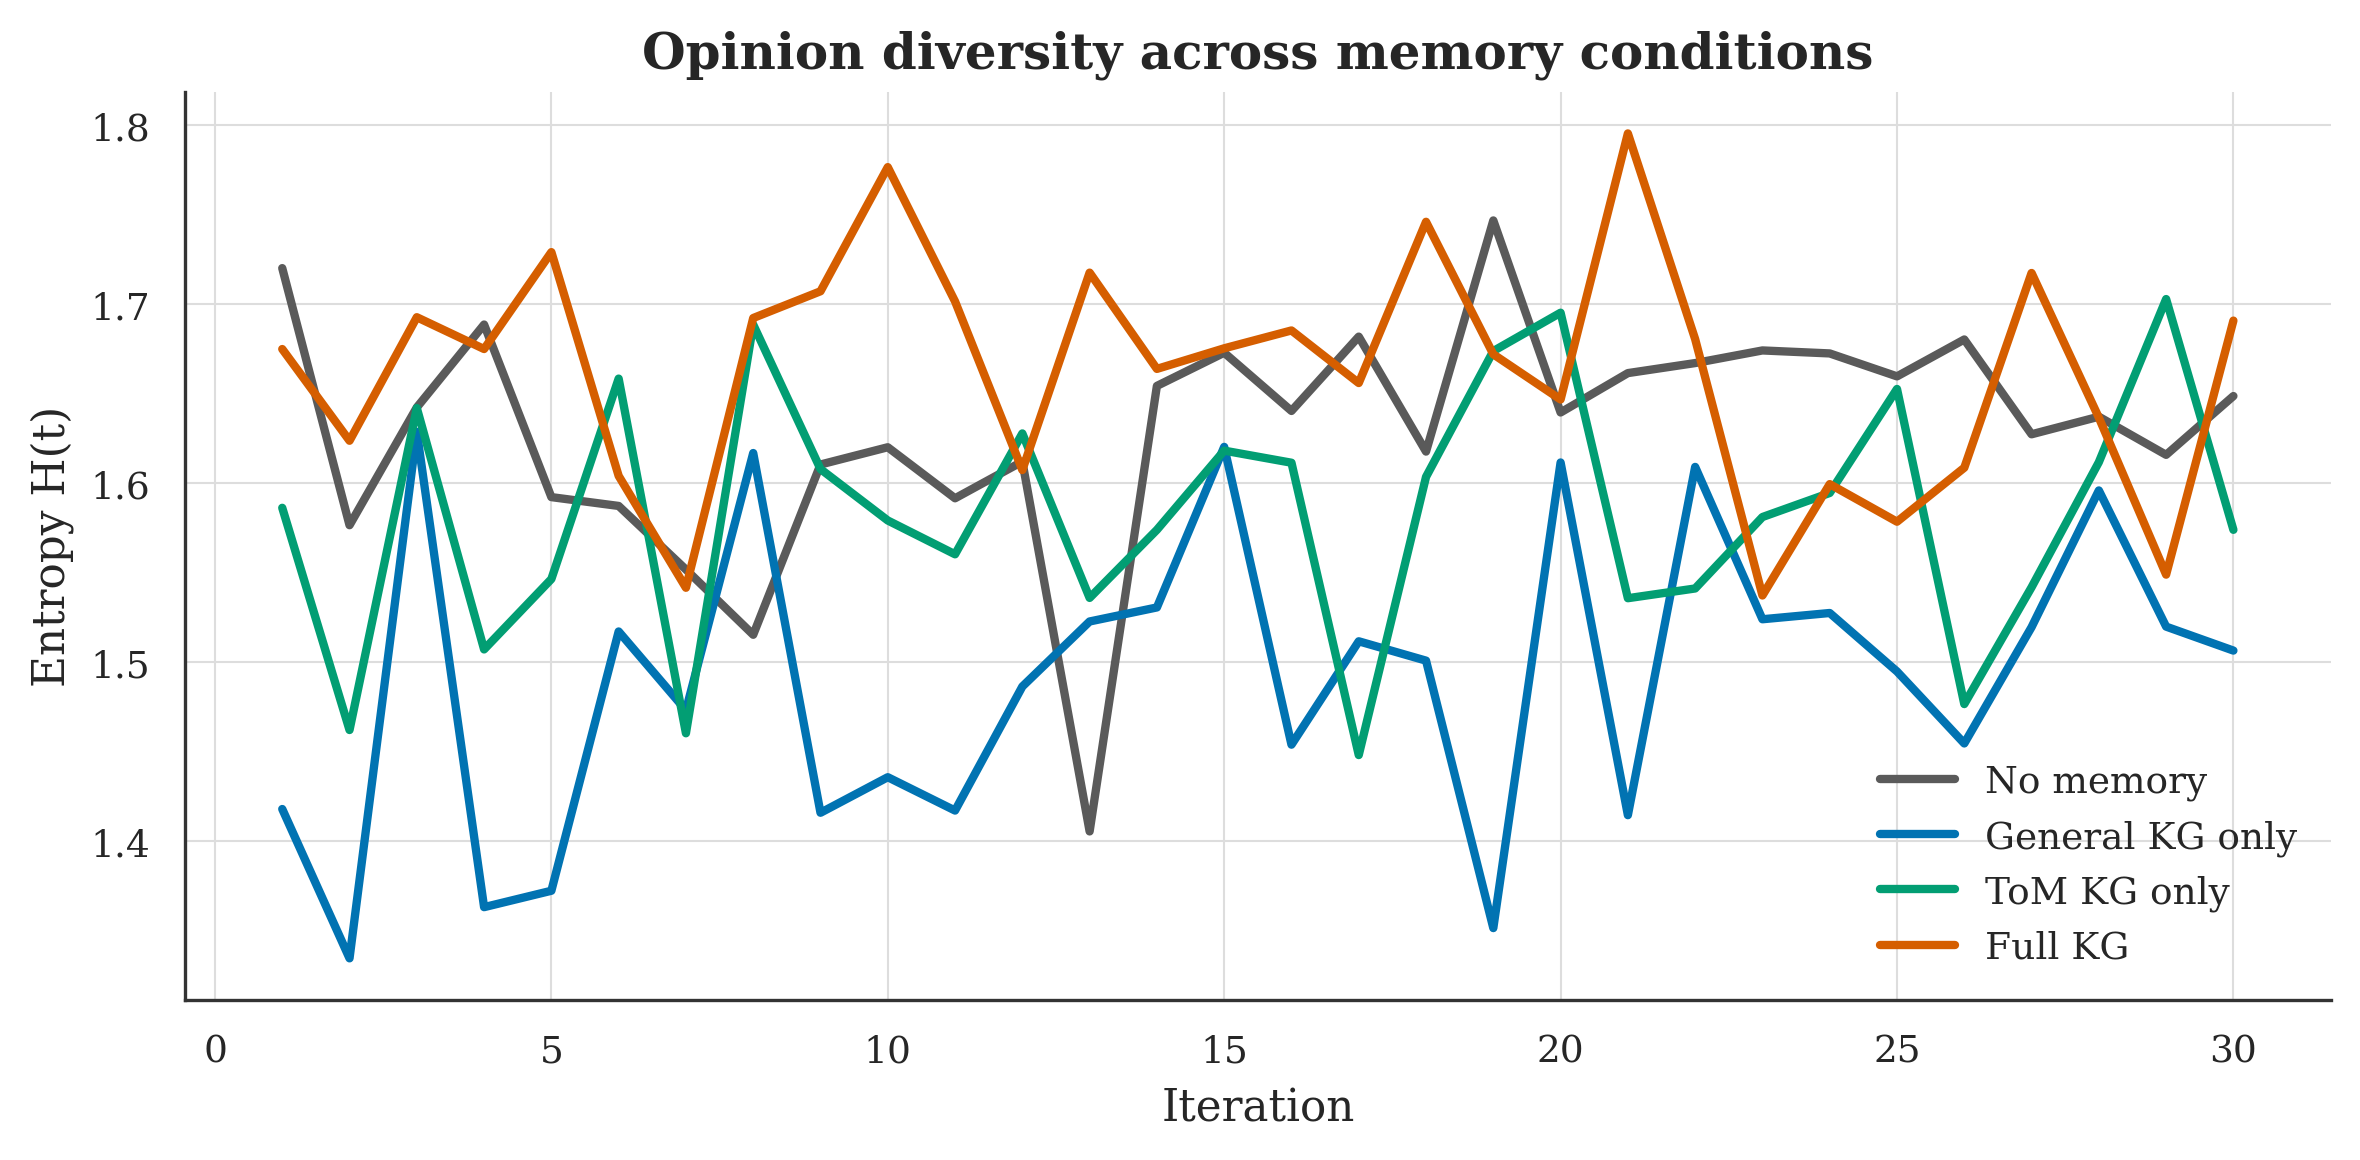
\includegraphics[width=\linewidth]{compare_entropy.png}
\caption{Shannon entropy $H(t)$ of the five-label stance distribution at the end of each simulated day, days 1 to 30, for the four memory conditions.}
\label{fig:entropy}
\end{figure}

\begin{figure}[t]
\centering
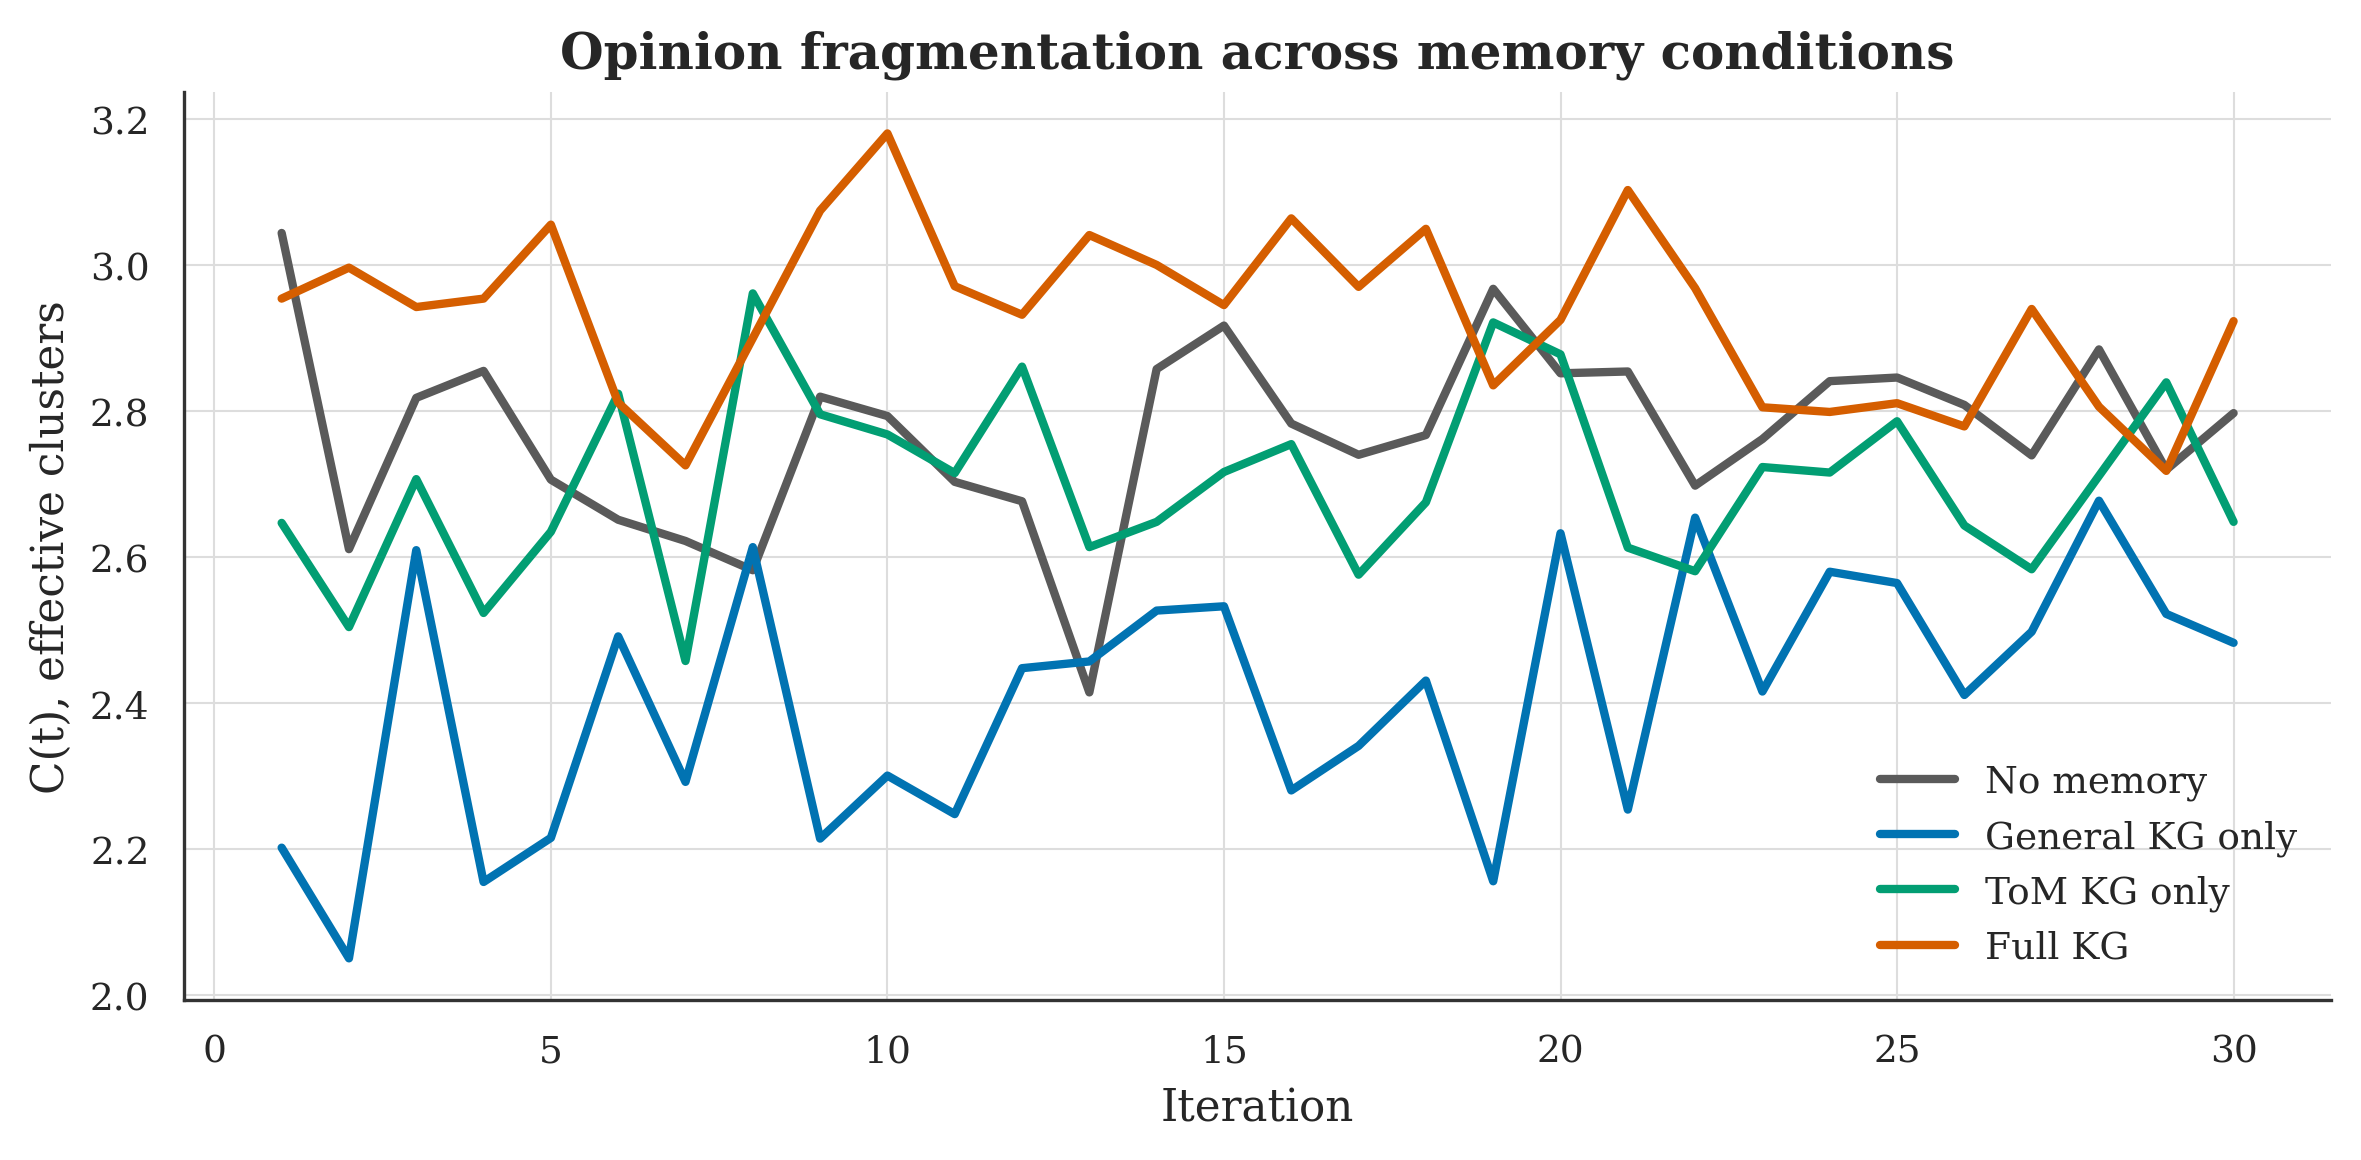
\includegraphics[width=\linewidth]{compare_effective_clusters.png}
\caption{Effective number of opinion clusters $C$ at the end of each simulated day, days 1 to 30.}
\label{fig:clusters}
\end{figure}

\begin{figure}[t]
\centering
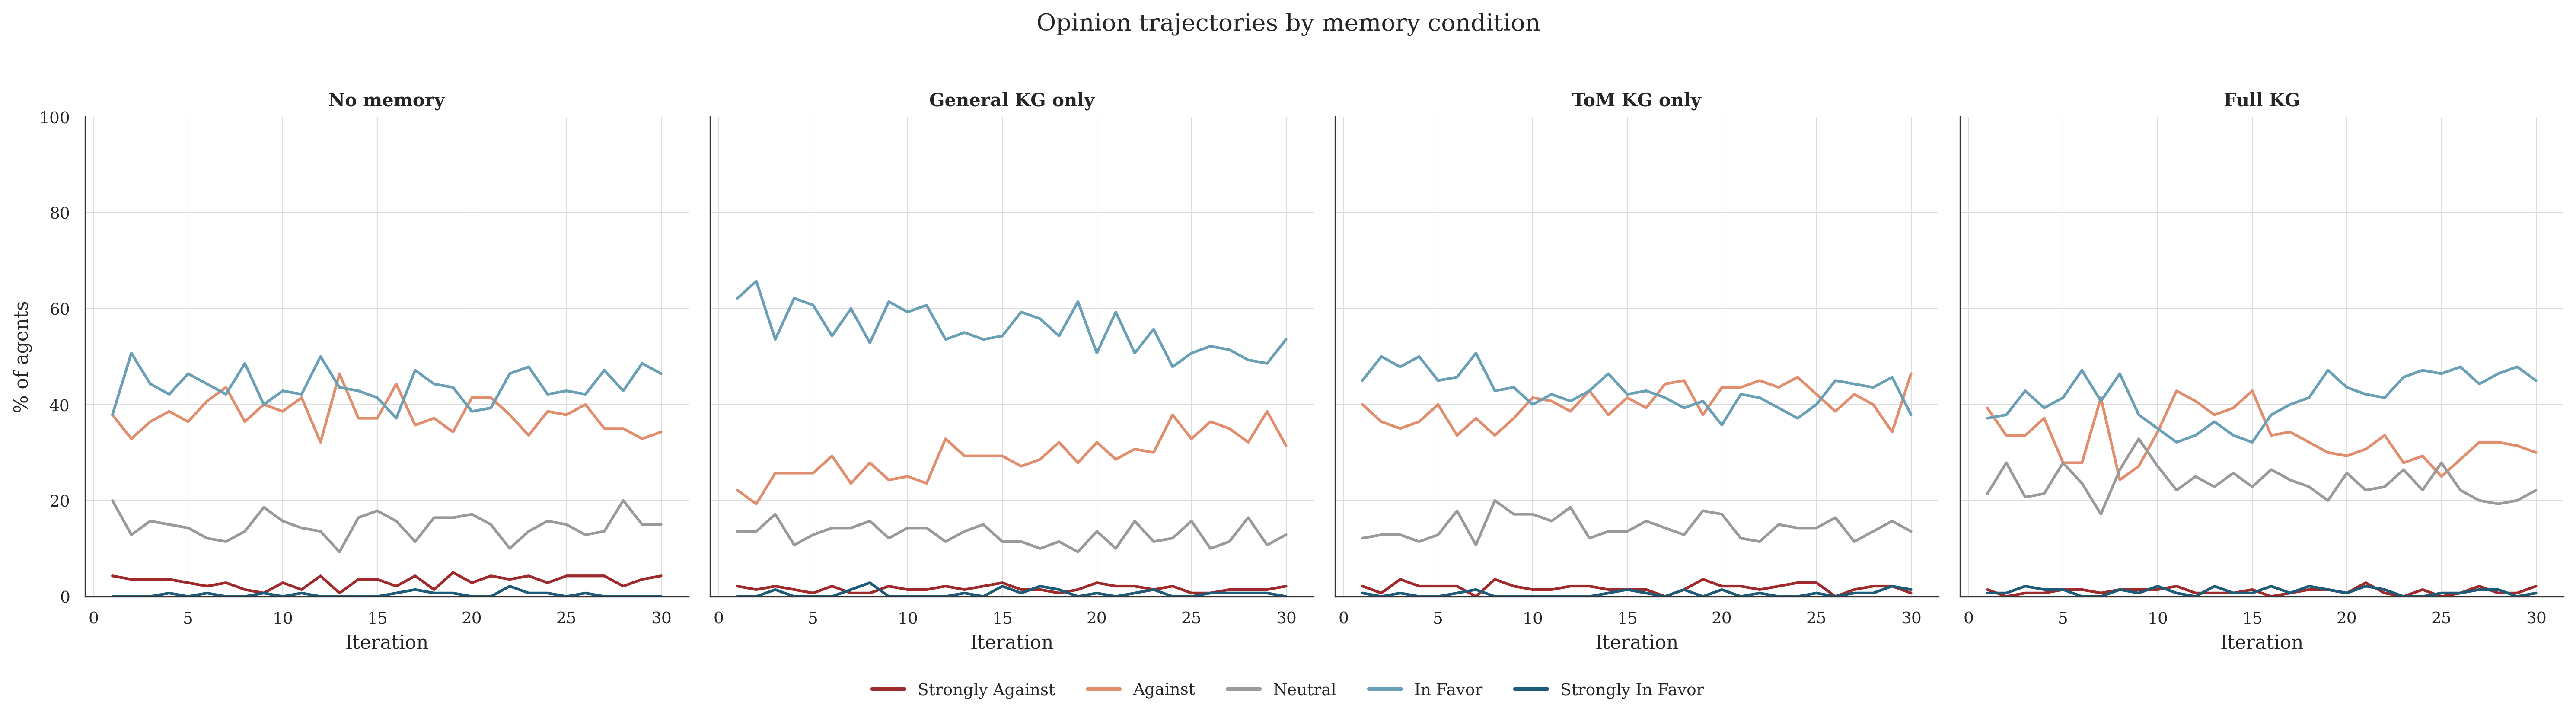
\includegraphics[width=\linewidth]{compare_trajectories.png}
\caption{Share of agents at each stance over the 30-day run, one panel per memory condition.}
\label{fig:trajectories}
\end{figure}

\subsection{Direction of drift}\label{sec:res-drift}
% GUIDE  Summary file, Section 2.3 and Section 4. general_only moves furthest
% GUIDE  toward In Favor (+0.179); tom_only is the only one below zero (-0.071);
% GUIDE  no_kg about 0 (+0.036). The pilot's left drift does NOT recur.
% GUIDE  Use scale labels only.
\pending{write}

\begin{table}[t]
\centering
\small
\caption{Neutral outflow.}
\label{tab:neutral}
\begin{tabular}{lcc}
\toprule
Condition & P(N to F) & P(N to A) \\
\midrule
\cond{no\_kg} & 0.437 & 0.438 \\
\cond{general\_only} & 0.519 & 0.335 \\
\cond{tom\_only} & 0.492 & 0.434 \\
\cond{full\_kg} & 0.470 & 0.448 \\
\bottomrule
\end{tabular}
\end{table}

\subsection{Selective agreement: signed distance}\label{sec:res-signed}
% GUIDE  Summary file, Section 3.4. One-step directional bias in every condition;
% GUIDE  about fourfold under general_only (+0.176 vs +0.042, non-overlapping
% GUIDE  intervals); only full_kg is positive at two steps (+0.062).
% GUIDE  Caveat: Delta x = +/-3 is confounded with extremes regressing to the centre.
\pending{write}

\begin{table}[t]
\centering
\small
\caption{Acceptance by signed distance $\Delta x$ (point estimate, n in parentheses).}
\label{tab:signed}
\resizebox{\linewidth}{!}{%
\begin{tabular}{lcccccc}
\toprule
Condition & $\Delta x = -3$ & $\Delta x = -2$ & $\Delta x = -1$ & $\Delta x = +1$ & $\Delta x = +2$ & $\Delta x = +3$ \\
\midrule
\cond{no\_kg} & 0.222 (3343) & 0.112 (33559) & 0.232 (28804) & 0.274 (28804) & 0.091 (33559) & 0.552 (3343) \\
\cond{general\_only} & 0.250 (2251) & 0.103 (32799) & 0.184 (24521) & 0.360 (24521) & 0.096 (32799) & 0.596 (2251) \\
\cond{tom\_only} & 0.263 (1947) & 0.132 (33928) & 0.249 (28740) & 0.301 (28740) & 0.098 (33928) & 0.557 (1947) \\
\cond{full\_kg} & 0.457 (1617) & 0.236 (27927) & 0.319 (37531) & 0.386 (37531) & 0.299 (27927) & 0.578 (1617) \\
\bottomrule
\end{tabular}}
\end{table}

\begin{table}[t]
\centering
\small
\caption{Directional asymmetry, agent-clustered bootstrap 95\% intervals.}
\label{tab:asymmetry}
\begin{tabular}{lcc}
\toprule
Condition & $P(A \mid {+}1) - P(A \mid {-}1)$ & $P(A \mid {+}2) - P(A \mid {-}2)$ \\
\midrule
\cond{no\_kg} & +0.042 [+0.013, +0.073] & -0.022 [-0.040, -0.002] \\
\cond{general\_only} & +0.176 [+0.145, +0.206] & -0.007 [-0.024, +0.009] \\
\cond{tom\_only} & +0.052 [+0.018, +0.084] & -0.034 [-0.053, -0.015] \\
\cond{full\_kg} & +0.067 [+0.040, +0.094] & +0.062 [+0.036, +0.089] \\
\bottomrule
\end{tabular}
\end{table}

\begin{figure}[t]
\centering
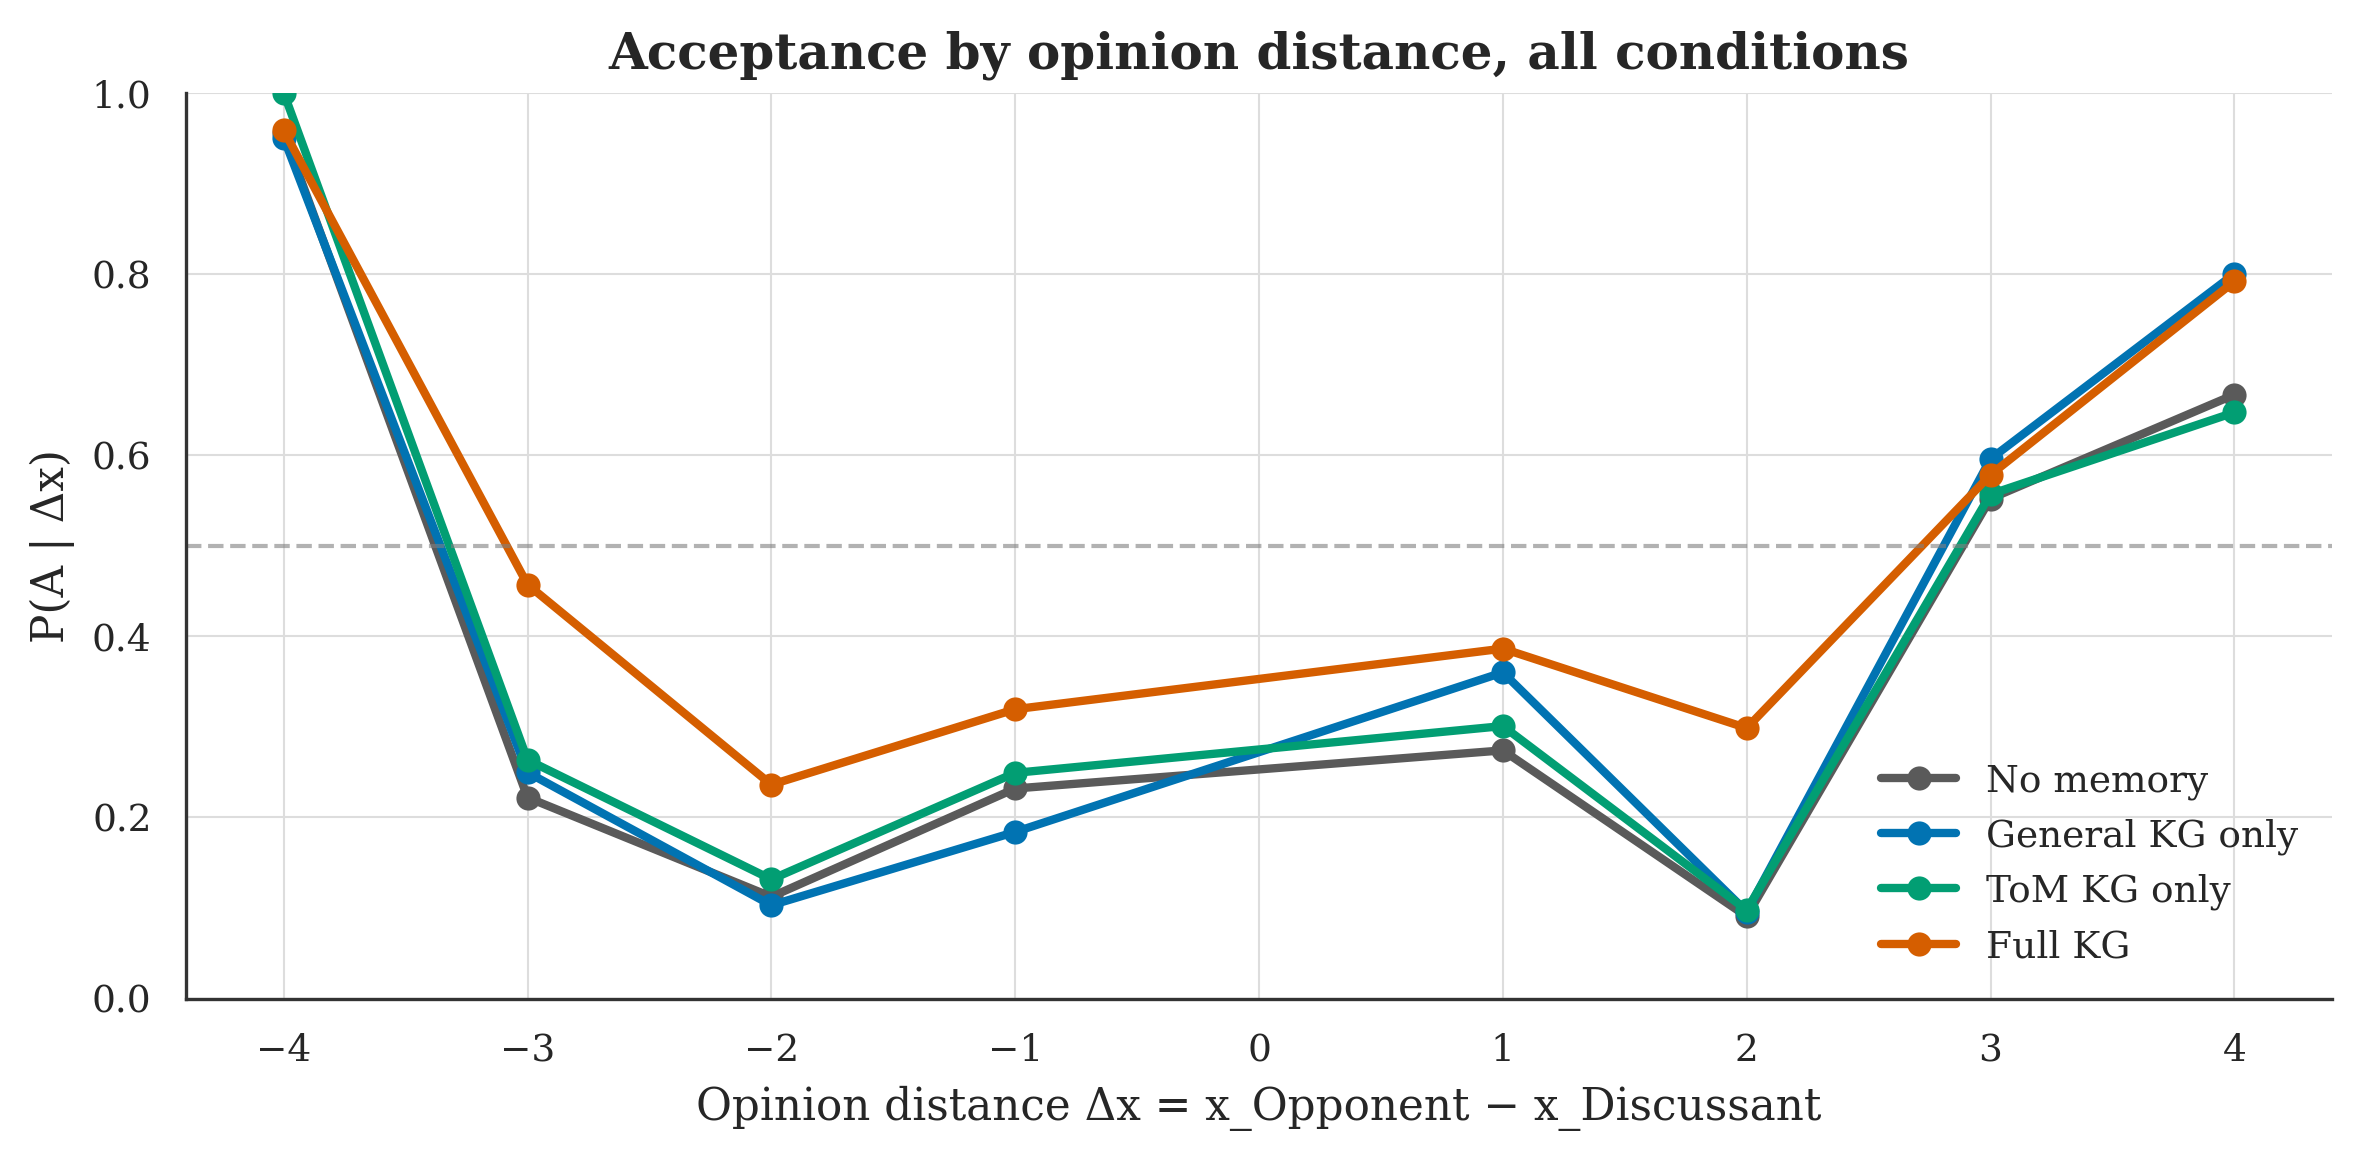
\includegraphics[width=\linewidth]{compare_acceptance_distance.png}
\caption{Acceptance probability $P(A \mid \Delta x)$ by signed opinion distance $\Delta x = x_{\mathrm{partner}} - x_{\mathrm{agent}}$, all four conditions. Values at $|\Delta x| \geq 3$ rest on few pairs and coincide with regression from the extremes (the unsigned-distance subsection).}
\label{fig:acceptance}
\end{figure}

\subsection{Sensitivity to distance: unsigned}\label{sec:res-unsigned}
% GUIDE  Summary file, Sections 3.1-3.2. Acceptance falls from d=1 to d=2
% GUIDE  everywhere; the d2/d1 ratio is 0.366-0.417 in three conditions and 0.758
% GUIDE  under full_kg. The flattening comes from MORE acceptance, not more
% GUIDE  resistance (move-away at d=2 is 0.025-0.042). d>=3 is confounded.
\pending{write}

\begin{table}[t]
\centering
\small
\caption{Acceptance by unsigned distance, agent-clustered bootstrap 95\% intervals.}
\label{tab:unsigned}
\resizebox{\linewidth}{!}{%
\begin{tabular}{lccccc}
\toprule
Condition & P(acc, $d = 1$) & P(acc, $d = 2$) & Ratio $d_2/d_1$ & P(away, $d = 1$) & P(away, $d = 2$) \\
\midrule
\cond{no\_kg} & 0.253 [0.243, 0.263] & 0.102 [0.092, 0.112] & 0.401 [0.373, 0.430] & 0.283 [0.268, 0.297] & 0.042 [0.032, 0.052] \\
\cond{general\_only} & 0.272 [0.262, 0.282] & 0.099 [0.092, 0.107] & 0.366 [0.346, 0.386] & 0.233 [0.222, 0.244] & 0.028 [0.020, 0.037] \\
\cond{tom\_only} & 0.275 [0.266, 0.283] & 0.115 [0.107, 0.123] & 0.417 [0.396, 0.438] & 0.283 [0.273, 0.294] & 0.025 [0.018, 0.032] \\
\cond{full\_kg} & 0.353 [0.346, 0.360] & 0.267 [0.257, 0.277] & 0.758 [0.740, 0.775] & 0.268 [0.262, 0.274] & 0.032 [0.026, 0.039] \\
\bottomrule
\end{tabular}}
\end{table}

\subsection{Mobility by starting stance}\label{sec:res-mobility}
% GUIDE  Summary file, Section 3.3. A and F are the stickiest; SF leaves in more
% GUIDE  than 90% of updates; SA in 62-73%; SA is least mobile under no_kg.
\pending{write}

\begin{table}[t]
\centering
\small
\caption{Mobility by starting stance.}
\label{tab:mobility}
\begin{tabular}{lcccc}
\toprule
Starting stance & \cond{no\_kg} & \cond{general\_only} & \cond{tom\_only} & \cond{full\_kg} \\
\midrule
SA & 0.620 & 0.695 & 0.647 & 0.731 \\
A & 0.237 & 0.195 & 0.215 & 0.367 \\
N & 0.875 & 0.853 & 0.926 & 0.919 \\
F & 0.178 & 0.139 & 0.199 & 0.293 \\
SF & 0.939 & 0.947 & 0.964 & 0.920 \\
\bottomrule
\end{tabular}
\end{table}

\subsection{The hypothesis, criterion by criterion}\label{sec:res-hypothesis}
% GUIDE  Use the table below (from the Outcome section of hypothesis_and_scope.md).
% GUIDE  Two points: (1) full_kg meets the entropy criterion but is the LEAST
% GUIDE  stable on every other measure, a reversal on stability; (2) tom_only
% GUIDE  changes the least (curve shape and asymmetry overlap no_kg; it raises
% GUIDE  d=1 acceptance slightly, 0.275 vs 0.253).
% GUIDE  Do not use the labels "Information Paradox" or "Memory Asymmetry Principle".
\pending{write}

\begin{table}[t]
\centering
\small
\caption{Criteria stated in advance, against the delivered results.}
\label{tab:criteria}
\begin{tabularx}{\linewidth}{>{\raggedright\arraybackslash}p{0.28\linewidth}>{\raggedright\arraybackslash}X>{\raggedright\arraybackslash}X}
\toprule
Criterion stated in advance & Result & Verdict \\
\midrule
Support: \cond{tom\_only} has a flatter acceptance-by-distance curve than \cond{no\_kg} and \cond{general\_only} & $d_2/d_1$ acceptance ratio: \cond{tom\_only} 0.417 [0.396, 0.438], \cond{no\_kg} 0.401 [0.373, 0.430], \cond{general\_only} 0.366 [0.346, 0.386] & Not supported. \cond{tom\_only} is indistinguishable from \cond{no\_kg} \\ \addlinespace
Support: \cond{full\_kg} has the smallest entropy change over the run & Entropy drop, day 0 to 30: \cond{full\_kg} 0.431, \cond{no\_kg} 0.473, \cond{tom\_only} 0.548, \cond{general\_only} 0.615 bits & Met as operationalised, but see the stability discussion below \\ \addlinespace
Support: \cond{general\_only} sits between \cond{no\_kg} and \cond{tom\_only}, or does not differ from \cond{no\_kg} & Acceptance curve close to \cond{no\_kg}; population outcome is the most convergent of all four & Mixed. No effect on the curve, largest effect on convergence \\ \addlinespace
Against: no KG condition moves the acceptance curve relative to \cond{no\_kg} & \cond{full\_kg} ratio 0.758 [0.740, 0.775] & Not met. \cond{full\_kg} clearly moves it \\ \addlinespace
Against: \cond{tom\_only} and \cond{general\_only} curves indistinguishable & $d = 1$ 0.275 vs 0.272; $d = 2$ 0.115 vs 0.099; ratio intervals do not overlap (0.417 vs 0.366) but both sit near \cond{no\_kg} & Largely met. Neither single-dimension memory changes selective agreement much \\ \addlinespace
Against: some KG condition has a larger entropy collapse than \cond{no\_kg} & \cond{general\_only} (0.615) and \cond{tom\_only} (0.548) both exceed \cond{no\_kg} (0.473) & Met for \cond{general\_only} and \cond{tom\_only} \\
\bottomrule
\end{tabularx}
\end{table}

% GUIDE  Optional subsection: the language-level numbers from Rossetti's external
% GUIDE  report (fallacy 38.9% full_kg vs 61.1% no_kg; NEVER 83.7%; sentiment
% GUIDE  ordering; concept overlap). Include only after he confirms provenance and
% GUIDE  shares the code; label it provisional. Several of that report's
% GUIDE  directional claims did not reproduce (summary file, Section 6).

% =============================================================================
\section{Discussion}\label{sec:discussion}
% GUIDE  Interpret ONLY what Results states; mark every mechanism as untested.
% GUIDE  Length: 1200-1700 words. Suggested subsections:
% GUIDE   - What kind of memory matters (facts: convergence + bias; combined:
% GUIDE     churn; ToM: little change).
% GUIDE   - Why general_only might amplify the bias. Candidate: accumulated facts
% GUIDE     lean one way. Untestable without the KG databases and transcripts.
% GUIDE   - Why full_kg churns: context volume, the beliefs dimension, or an
% GUIDE     annotator effect. The design cannot separate them.
% GUIDE   - The reversal: an entropy criterion cannot tell stable individuals from
% GUIDE     a churning population whose aggregate stays diverse.
% GUIDE   - Relation to LODAS: the directional bias appears even without memory;
% GUIDE     analogous to Cau et al., not the same measurement (no stated proposition).
% GUIDE   - Next experiments, in priority order: more seeds; an explicit
% GUIDE     proposition under both framings; KG and transcript analysis of the
% GUIDE     existing runs; an annotator control.
\pending{write}

% =============================================================================
\section{Limitations}\label{sec:limitations}
% GUIDE  One paragraph per limitation, stated plainly. Length: 700-1000 words.
% GUIDE  One run per condition (LODAS used 10); one topic; one unconfirmed model;
% GUIDE  no stated proposition; annotator is a model judgment (a design difference
% GUIDE  from LODAS, not a shared limitation); clamp and scale edges; cadence loop
% GUIDE  unconfirmed (affects FSRS decay); untuned FSRS; 140 agents with random
% GUIDE  pairing and no network; the "stated in advance" criterion was a poor proxy;
% GUIDE  external language analyses are not reproducible.
\pending{write}

% =============================================================================
\section{Conclusion}\label{sec:conclusion}
% GUIDE  300-450 words, no new claims: what you did, the three findings, what this
% GUIDE  does not establish, and the next experiments. Do not start with "In conclusion".
\pending{write}

% =============================================================================
\section*{Data and code availability}
\pending{repository URL and release decision; whether transcripts and KG databases can be shared}

\section*{Author contributions}
\pending{to be agreed}

\section*{Competing interests}
\pending{to be confirmed}

\section*{Acknowledgements}
\pending{DGX compute, funding}

% \nocite{*} lists every verified reference so you can see what is available
% while writing. REMOVE it before submission, so that only cited works appear.
\nocite{*}
\bibliographystyle{plainnat}
\bibliography{references}

\end{document}
